\subsection{Tại Sao Tuyến Tính Mang Lại Lợi Thế}
% -----------------------------------------------------------------------------

Tính tuyến tính trong tham số không phải là giả định tùy tiện. Nó cung cấp ba lợi thế cụ thể, tất cả đều bắt nguồn từ cùng một tính chất cấu trúc: $\hat{\boldsymbol{\beta}}$ là \textbf{tổ hợp tuyến tính của $\mathbf{y}$}.

\textbf{1. Nghiệm dạng đóng.}
\textit{Nghiệm dạng đóng} (closed-form solution) nghĩa là bài toán có một công thức đại số hữu hạn để tính trực tiếp kết quả, thay vì phải dò nghiệm bằng thuật toán lặp \cite[Sec.~2.4]{weisberg2014applied}. Với OLS, mục tiêu là chọn $\boldsymbol{\beta}$ để tối thiểu hóa tổng bình phương phần dư:
\[
  RSS(\boldsymbol{\beta})
  = (\mathbf{y} - \mathbf{X}\boldsymbol{\beta})^\top
    (\mathbf{y} - \mathbf{X}\boldsymbol{\beta}).
\]

Vì mô hình tuyến tính trong $\boldsymbol{\beta}$, hàm $RSS(\boldsymbol{\beta})$ là một hàm bậc hai theo các tham số. Lấy đạo hàm theo $\boldsymbol{\beta}$ và cho bằng 0 tạo ra \textbf{hệ phương trình chuẩn}:
\[
  \mathbf{X}^\top\mathbf{X}\,\hat{\boldsymbol{\beta}}
  = \mathbf{X}^\top\mathbf{y}.
\]
Góc nhìn hình học tương đương là phần dư $\mathbf{e}=\mathbf{y}-\mathbf{X}\hat{\boldsymbol{\beta}}$ phải trực giao với mọi cột của $\mathbf{X}$, tức $\mathbf{X}^\top\mathbf{e}=0$.

Nếu $\mathbf{X}$ đầy đủ hạng cột, $\mathbf{X}^\top\mathbf{X}$ khả nghịch và ta cô lập được nghiệm:
\[
  \hat{\boldsymbol{\beta}}
  = (\mathbf{X}^\top\mathbf{X})^{-1}\mathbf{X}^\top\mathbf{y}.
\]
Đây là nghiệm dạng đóng của OLS: về mặt toán học, nó cho nghiệm duy nhất và là cực tiểu toàn cục của RSS. Trong tính toán thực tế, phần mềm thường dùng các phân rã số như QR hoặc Cholesky thay vì nghịch đảo ma trận trực tiếp, nhưng bản chất vẫn là giải hệ tuyến tính một lần, không phải dò lặp như hồi quy phi tuyến.


Nếu $\mathbf{X}$ không đầy đủ hạng cột, thường do đa cộng tuyến hoàn hảo, thì $\mathbf{X}^\top\mathbf{X}$ không khả nghịch và công thức nghịch đảo ở trên không áp dụng. Khi đó hệ phương trình chuẩn có thể có vô số nghiệm; các cách xử lý chuẩn gồm dùng generalized inverse, đặt side conditions, hoặc tái tham số hóa mô hình \cite[Ch.~12, p.~302]{rencher2008linear}. Nếu mục tiêu chính là ổn định dự báo trong bối cảnh đa cộng tuyến mạnh, các phương pháp regularization như ridge hoặc lasso cũng là lựa chọn thực hành \cite[Sec.~10.2.3, p.~244]{weisberg2014applied}.

\textbf{2. Ước lượng tối ưu---Định lý Gauss-Markov.}
Vì $\hat{\boldsymbol{\beta}}$ là tổ hợp tuyến tính của $\mathbf{y}$, trong lớp tất cả các ước lượng tuyến tính không chệch, OLS đạt phương sai nhỏ nhất---tính chất \textbf{BLUE} (Best Linear Unbiased Estimator) \cite[Thm.~7.3d, p.~145]{rencher2008linear}. Định lý này không đòi hỏi phân phối chuẩn: chỉ cần $E(\varepsilon|X)=0$, $\mathrm{Var}(\varepsilon)=\sigma^2 I$, và $\mathrm{Cov}(\varepsilon_i,\varepsilon_j)=0$.

\textbf{3. Suy diễn đáng tin---Định lý Giới Hạn Trung Tâm cho $\hat{\boldsymbol{\beta}}$.}
Vì $\hat{\boldsymbol{\beta}}$ là tổ hợp tuyến tính của $\mathbf{y}$, CLT đảm bảo $\hat{\boldsymbol{\beta}}$ xấp xỉ chuẩn trong mẫu lớn dù sai số có phân phối bất kỳ. Khi sai số \textit{thực sự} chuẩn, $\hat{\boldsymbol{\beta}}$ chuẩn chính xác và thống kê $t$, $F$ theo đúng phân phối lý thuyết---nền tảng của mọi kiểm định giả thuyết và khoảng tin cậy.

\begin{figure}[H]
  \centering
  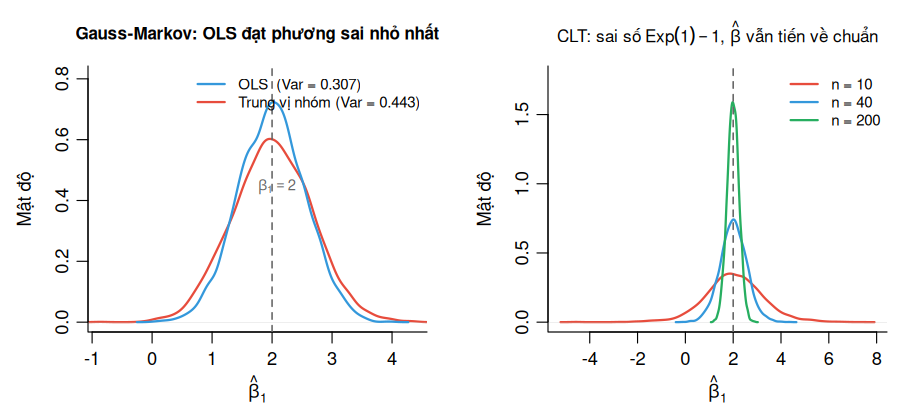
\includegraphics[width=\textwidth]{./figures/fig6_blue_clt.png}
  \caption{Minh họa hai lợi thế của tuyến tính trong tham số.
  \textbf{Trái (Gauss-Markov BLUE):} $B = 4000$ lần mô phỏng, $n=40$, $\beta_1 = 2$.
  OLS (xanh dương) có phân phối lấy mẫu hẹp hơn đáng kể so với ước lượng tuyến tính không chệch thay thế (đỏ), cả hai đều tập trung tại giá trị thực.
  \textbf{Phải (CLT cho $\hat{\beta}_1$):} sai số có phân phối $\mathrm{Exp}(1) - 1$ lệch phải rõ ràng.
  Khi $n$ tăng từ 10 lên 200, phân phối lấy mẫu của $\hat{\beta}_1$ nhanh chóng tiến về chuẩn---suy diễn bằng $t$-test vẫn hợp lệ tiệm cận.}
  \label{fig:blue_clt}
\end{figure}

% -----------------------------------------------------------------------------
